\documentclass{beamer}[10]

\usepackage{graphicx}
\usepackage{xcolor}
\usepackage{tabto}
%\usepackage{beamerthemesplit}
\usepackage{tikz}
\usepackage{cancel}
\usepackage{verbatim}
\usepackage{fancybox}
\usepackage{enumerate}
\usepackage{amsmath,amssymb,amsthm,textcomp,mathtools}
\usepackage[super]{nth}
\usepackage[amssymb]{SIunits}
\usepackage{booktabs}
\usepackage{cancel}
\usepackage{bm}
\usepackage[utf8]{inputenc}
\usepackage{tabularx}
\usepackage{ragged2e}
\newcolumntype{Y}{ >{\RaggedRight\arraybackslash}X}
\usetikzlibrary{arrows,shapes}
\newcommand\T{\rule{0pt}{2.6ex}}
\newcommand\B{\rule[-1.2ex]{0pt}{0pt}}
\definecolor{UUcrimson}{RGB}{204,0,0}
\mode<presentation>
{ \usetheme{default}
  \usecolortheme[named=UUcrimson]{structure}
  \useinnertheme{circles}
  \setbeamercovered{transparent}
  \setbeamertemplate{blocks}[rounded]
  \usefonttheme[onlymath]{serif}
  \setbeamertemplate{navigation symbols}{}
  \setbeamertemplate{footline}[page number]
  \setbeamertemplate{navigation symbols}{}
  \setbeamercolor{section in toc}{fg=black,bg=white}
  \setbeamercolor{alerted text}{fg=UUcrimson!80!gray}
  \setbeamercolor*{palette primary}{fg=white,bg=UUcrimson}
  \setbeamercolor*{palette secondary}{fg=UUcrimson!70!black,bg=gray!15!white}
  \setbeamercolor*{palette tertiary}{bg=UUcrimson!80!black,fg=gray!10!white}
  \setbeamercolor*{palette quaternary}{fg=UUcrimson,bg=gray!5!white}
  \setbeamercolor*{palette sidebar primary}{fg=UUcrimson!10!black}
  \setbeamercolor*{palette sidebar secondary}{fg=white}
  \setbeamercolor*{palette sidebar tertiary}{fg=UUcrimson!50!black}
  \setbeamercolor*{palette sidebar quaternary}{fg=gray!10!white}
  \setbeamercolor{titlelike}{parent=palette primary,fg=white}
  \setbeamercolor{frametitle}{bg=UUcrimson}
  \setbeamercolor{frametitle right}{bg=UUcrimson}
  \setbeamercolor*{separation line}{}
  \setbeamercolor*{fine separation line}{}
}

\usetikzlibrary{backgrounds}
\makeatletter
\tikzstyle{every picture}+=[remember picture]
\tikzset{%
  fancy quotes/.style={
    text width=\fq@width pt,
    align=justify,
    inner sep=1em,
    anchor=north west,
    minimum width=\linewidth,
    font=\itshape
  },
  fancy quotes width/.initial={.8\linewidth},
  fancy quotes marks/.style={
    scale=8,
    text=white,
    inner sep=0pt,
  },
  fancy quotes opening/.style={
    fancy quotes marks,
  },
  fancy quotes closing/.style={
    fancy quotes marks,
  },
  fancy quotes background/.style={
    show background rectangle,
    inner frame xsep=0pt,
    background rectangle/.style={
      fill=gray!25,
      rounded corners,
    },
  }
}
\newenvironment{fancyquotes}[1][]{%
\noindent
\tikzpicture[fancy quotes background]
\node[fancy quotes opening,anchor=north west] (fq@ul) at (0,0) {``};
\tikz@scan@one@point\pgfutil@firstofone(fq@ul.east)
\pgfmathsetmacro{\fq@width}{\linewidth - 2*\pgf@x}
\node[fancy quotes,#1] (fq@txt) at (fq@ul.north west) \bgroup}
{\egroup;
\node[overlay,fancy quotes closing,anchor=east] at (fq@txt.south east) {''};
\endtikzpicture}
\makeatother


\usetikzlibrary{backgrounds}
\makeatletter
\tikzstyle{every picture}+=[remember picture]
\tikzset{%
  fancy defs/.style={
    text width=\fq@width pt,
    align=justify,
    inner sep=0.25em,
    anchor=north west,
    minimum width=\linewidth,
    font=\itshape
  },
  fancy defs width/.initial={.8\linewidth},
  fancy defs marks/.style={
    scale=8,
    text=white,
    inner sep=0pt,
  },
  fancy defs opening/.style={
    fancy defs marks,
  },
  fancy defs closing/.style={
    fancy defs marks,
  },
  fancy defs background/.style={
    show background rectangle,
    inner frame xsep=0pt,
    background rectangle/.style={
      fill=gray!25,
      rounded corners,
    },
  }
}
\newenvironment{fancydefs}[1][]{%
\noindent
\tikzpicture[fancy defs background]
\node[fancy defs opening,anchor=north west] (fq@ul) at (0,0) {};
\tikz@scan@one@point\pgfutil@firstofone(fq@ul.east)
\pgfmathsetmacro{\fq@width}{\linewidth - 2*\pgf@x}
\node[fancy defs,#1] (fq@txt) at (fq@ul.north west) \bgroup}
{\egroup;
\node[overlay,fancy defs closing,anchor=east] at (fq@txt.south east) {};
\endtikzpicture}
\makeatother
\usepackage{scalerel}[2014/03/10]
\usepackage{stackengine}
\usepackage{empheq}
\newcommand*\widefbox[1]{\fbox{\hspace{0.5em}#1\hspace{0.5em}}}

\newcommand\reallywidetilde[1]{\ThisStyle{%
  \setbox0=\hbox{$\SavedStyle#1$}%
  \stackengine{-.1\LMpt}{$\SavedStyle#1$}{%
    \stretchto{\scaleto{\SavedStyle\mkern.2mu\sim}{.5467\wd0}}{.4\ht0}%
%    .2mu is the kern imbalance when clipping white space
%    .5467++++ is \ht/[kerned \wd] aspect ratio for \sim glyph
  }{O}{c}{F}{T}{S}%
}}
\usepackage{media9}

\logo{
\includegraphics[width=0.75cm]{logo.jpg}}
\author[Gibbs]{Dr. Jeremy A. Gibbs}
\institute{Department of Mechanical Engineering\\University of Utah}
\date{Spring 2017}
\title{Environmental Fluid Dynamics: Lecture 15}
% colors
\newcommand{\ihat}{\boldsymbol{\hat{\imath}}}
\newcommand{\jhat}{\boldsymbol{\hat{\jmath}}}
\newcommand{\khat}{\boldsymbol{\hat{k}}}
\definecolor{colororange}{HTML}{E65100} % orange
\definecolor{colordgray}{HTML}{795548} % dark gray for note
\definecolor{colorhgray}{HTML}{212121} % heavy dark gray for normal text
\definecolor{colorgreen}{HTML}{009688} % green
\definecolor{colorwhite}{HTML}{FFFFFF} % background white
\definecolor{colorlgray}{HTML}{F5F3EE} % background light gray
\definecolor{colorblue}{HTML}{0277BB} % blue
\definecolor{colorred}{HTML}{CC0000} % red
\newcommand{\fontsizeone}{1.9em}
\setbeamertemplate{caption}{\raggedright\insertcaption\par}
\newcommand{\framecard}[2][colorgreen]{
  {\setbeamercolor{background canvas}{bg=#1}
    \begin{frame}[plain]
    \vfill
    \begin{center}
     {#2}
    \end{center}
    \vfill
    \end{frame}
  }
}
\begin{document}

%----------------------------------------------------------------------------------------
%	TITLE & TOC SLIDES
%----------------------------------------------------------------------------------------

\begin{frame} 
  \titlepage
\end{frame}

%------------------------------------------------

\begin{frame}
\frametitle{Overview}
\tableofcontents
\end{frame}
%------------------------------------------------
\section{Intro to Turbulence}                   %
%------------------------------------------------
\framecard[colorred]{{\color{white}\Huge Intro to Turbulence}}
%------------------------------------------------

\begin{frame}{Leonardo da Vinci and Turbulence}

\setlength{\fboxsep}{0pt}
\setlength{\fboxrule}{1pt}
\begin{columns}[T]
    \begin{column}{.6\textwidth}
      \begin{minipage}[c][.6\textheight][c]{\linewidth}
      \begin{itemize}
      \item Lived from 1452--1519. 
      \item First to attempt scientific study of turbulence (\textit{turbolenza}). 
      \item He pioneered the notion of flow visualization to study turbulence. 
      \end{itemize}
      \end{minipage}
    \end{column}
    \begin{column}{.4\textwidth}
    \fbox{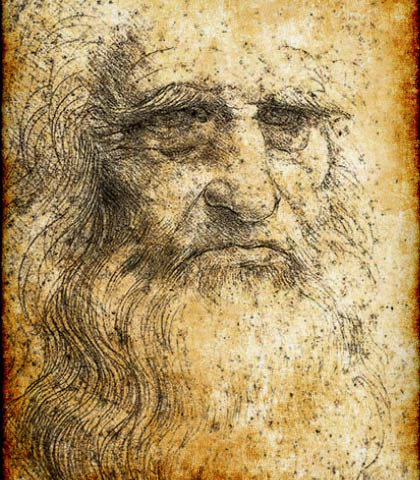
\includegraphics[width=\textwidth]{davinci1.jpg}}
    \end{column}
  \end{columns}

\end{frame}

%------------------------------------------------

\begin{frame}{Leonardo da Vinci and Turbulence}
  \setlength{\fboxsep}{0pt}
  \setlength{\fboxrule}{1pt}
  \begin{figure}[H]
  \centering
  \fbox{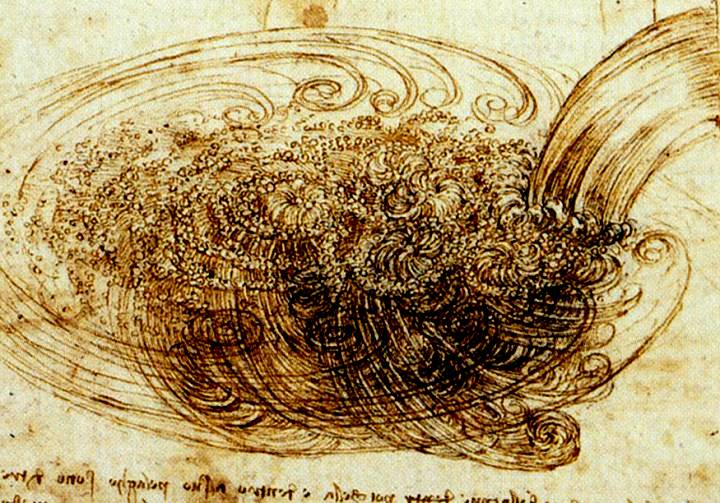
\includegraphics[width=0.4\textwidth]{davinci2.jpg}}
  \end{figure}
  
  He let water flow through a square hole into a pool and observed:
      \begin{fancyquotes}
      Observe the motion of the surface of the water, which resembles that of hair, which has two motions, of which one is caused by the weight of the hair, the other by the direction of the curls; thus the water has eddying motions, one part of which is due to the principal current, the other to random and reverse motion.	
      \end{fancyquotes}

Sounds very similar to Reynolds decomposition!

\end{frame}

%------------------------------------------------
\subsection{History}
\begin{frame}{Leonardo da Vinci and Turbulence}
  \setlength{\fboxsep}{0pt}
  \setlength{\fboxrule}{1pt}
  \begin{figure}[H]
  \centering
  \fbox{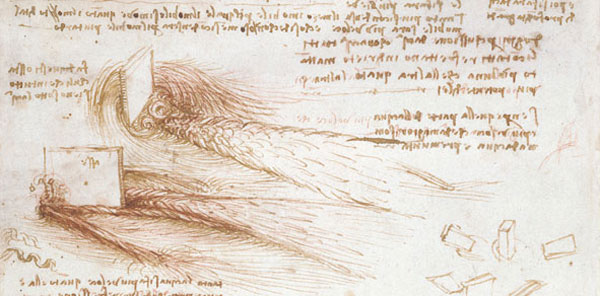
\includegraphics[width=0.5\textwidth]{davinci3.jpg}}
  \end{figure}
  
  In another, he placed obstacles in water:
      \begin{fancyquotes}
      So moving water strives to maintain the course pursuant to the power which occasions it, and if it finds an obstacle in its path it completes the span of the course it has commenced by a circular and revolving movement.	
      \end{fancyquotes}
Earliest reference to the importance of vortices!
\end{frame}

%------------------------------------------------

\begin{frame}{Leonardo da Vinci and Turbulence}
  \setlength{\fboxsep}{0pt}
  \setlength{\fboxrule}{1pt}
  \begin{figure}[H]
  \centering
  \fbox{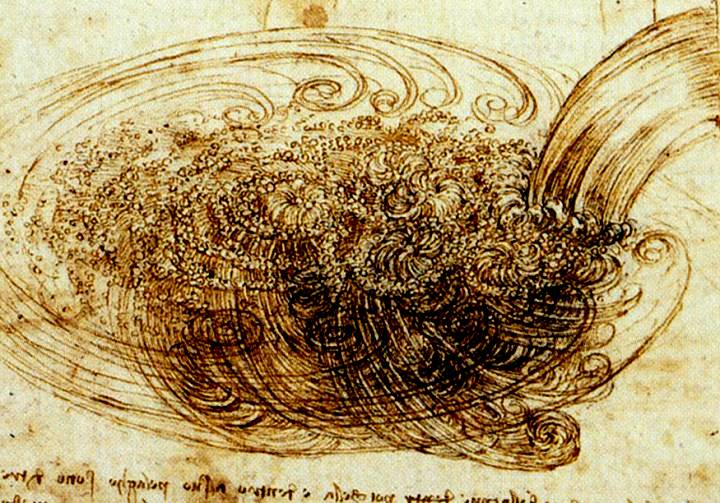
\includegraphics[width=0.5\textwidth]{davinci2.jpg}}
  \end{figure}
  
  In another, he placed obstacles in water:
      \begin{fancyquotes}
      ... the smallest eddies are almost numberless, and large things are rotated only by large eddies and not by small ones, and small things are turned by small eddies and large.	
      \end{fancyquotes}
Seems to hint at Richardson's turbulent cascade!
\end{frame}

%------------------------------------------------
\subsection{Motivation}
\begin{frame}{Why Turbulence?}

Why study turbulence?

\begin{itemize}
\item Turbulence is everywhere.
\item Smoke from a chimney, water flowing in a river, wind across a rough surface, flow around vehicles, combustion, solar wind.
\item Most real flows in environmental and engineering applications are turbulent. 
\item It remains one of the great unsolved problems in physics.
\end{itemize}

\end{frame}

%------------------------------------------------

\begin{frame}{Turbulence is Hard}

Werner Heisenberg, maybe:
\begin{fancyquotes}
	When I meet God, I am going to ask him two questions: Why relativity? And why turbulence? I really believe he will have an answer for the first.
\end{fancyquotes}

Horace Lamb, maybe:
\begin{fancyquotes}
	I am an old man now, and when I die and go to heaven there are two matters on which I hope for enlightenment. One is quantum electrodynamics, and the other is the turbulent motion of fluids. And about the former I am rather optimistic.
\end{fancyquotes}

\end{frame}
%------------------------------------------------
\begin{frame}{What Makes Turbulence Such a Difficult Problem?}
  Beyond these properties, consider turbulent flow in general.
  \begin{itemize}
  \item To understand turbulence, we must resolve the entire range of temporal and spatial scales of the flow. 
  \item This range may be described by the Reynolds number (Re=$UL/\nu$) -- the ratio of inertia to viscous forces.  
  \item As Re increases, the range of length scales that must be increases dramatically.
  \end{itemize}
\end{frame}

%------------------------------------------------

\begin{frame}{What Makes Turbulence Such a Difficult Problem?}
  
  These scales often fall outside of those conditions that are easily measured:
  \begin{itemize}
  	\item high-velocities (aerodynamics)
  	\item high-temperatures (combustion)
  	\item hazardous substances (nuclear engineering)
  	\item very large scales (geophysics or astrophysics)
  \end{itemize}
  ~\\~\\
   
\end{frame}

%------------------------------------------------

\begin{frame}{Approaches to Study Turbulence}
  
  Some common approaches to studying turbulence
  \begin{itemize}
  	\item \textbf{Analytical} \newline Due to the large range of scales and complexity of the flow, it is difficult (impossible really) to obtain an analytical solution
  	\item \textbf{Computational} \newline If we have large enough computing resources to resolve all scales of motion, we can solve the Navier-Stokes equations directly (DNS)
  	\item \textbf{Empirical} \newline Describing turbulence in a statistical framework
  \end{itemize}
\end{frame}

%------------------------------------------------

\begin{frame}{Approaches to Study Turbulence: Analytical}
  
  The Komogorov scales (more later) are defined as
  \begin{itemize}
		\item length scale $$\eta = \left(\frac{\nu^3}{\epsilon}\right)^{\frac{1}{4}}$$
		\item time scale $$\tau = \left(\frac{\nu}{\epsilon}\right)^{\frac{1}{2}}$$
		\item velocity scale $$v = \frac{\eta}{\nu} = (\nu \epsilon)^{\frac{1}{4}}$$
	\end{itemize}
	We can relate these to the Reynolds number as
	\begin{align*}
		\eta &\sim \ell_o \text{Re}^{-\frac{3}{4}}\\
		v &\sim U_o \text{Re}^{-\frac{1}{4}}\\
		\tau &\sim \frac{\ell_o}{U_o} \text{Re}^{-\frac{1}{2}}
	\end{align*}
\end{frame}
%------------------------------------------------

\begin{frame}{Approaches to Study Turbulence: Analytical}
\begin{itemize}
	\item Consider typical atmospheric scales:$$U_o\sim10\ \metre\ \reciprocal\second,\ \ell_o\sim10^3\ \metre,\ \nu \sim 10^{-5}\ \square\metre\ \reciprocal\second$$
	\item which gives us, $$\text{Re} = \frac{U_o \ell_o}{\nu} \sim \frac{(10\ \metre\ \reciprocal\second)(10^3\ \metre)}{10^{-5}\ \square\metre\ \reciprocal\second} \sim 10^9$$
	\item thus, 
	\begin{align*}
		\eta &\sim \ell_o \text{Re}^{-\frac{3}{4}} \sim 0.00018\ \metre \\
		v &\sim U_o \text{Re}^{-\frac{1}{4}} \sim 0.06\ \metre\ \reciprocal\second \\
		\tau &\sim \frac{\ell_o}{U_o} \text{Re}^{-\frac{1}{2}} \sim 0.003\ \second
	\end{align*}
\end{itemize}
That is quite the range of scales!	
\end{frame}

%------------------------------------------------

\begin{frame}{Approaches to Study Turbulence: Analytical}
\begin{itemize}
	\item Beyond the large range of scales that must be described, think about the complexity of flows
	\item For an analytical solution, we would have to understand and describe all of those situations
	\item Okay, let's try brute force!
\end{itemize}
\end{frame}

%------------------------------------------------

\begin{frame}{Approaches to Study Turbulence: Computational}

\begin{itemize}
	\item To capture all of the dynamics (degrees of freedom) in a turbulent flow, we must consider the required amount of discrete values needed for an accurate approximation.
	\item We need a grid fine enough to capture the smallest \textit{and} the largest scales of motion ($\eta$ and $\ell_o$).
\end{itemize}
\end{frame}

%------------------------------------------------

\begin{frame}{Approaches to Study Turbulence: Computational}

\begin{itemize}
	\item From K41, we know that $\ell_o/\eta\sim \text{Re}^{3/4}$ and there exists a continuous range of scales between $\eta$ and $\ell_o$.
	\item We will assume that we need $n$ grid points per increment $\eta$. Note that $n$ can vary, but a value of 3 to 5 is often suggested.
	\item Thus, in each direction, the number of required grid points is
	$$N_i = \frac{\ell_o}{(\eta/n)} = n\ \frac{\ell_o}{\eta} \sim n\ \text{Re}^{3/4}$$
	\item Remember that turbulence is 3D, so the total number of grid points needed to accurately estimate the flow is
	$$N = \left(n\ \text{Re}^{3/4} \right)^3 = \boxed{n^3\ \text{Re}^{9/4}}$$
\end{itemize}
\end{frame}


%------------------------------------------------

\begin{frame}{Approaches to Study Turbulence: Computational}

\begin{itemize}
	\item Let's revisit our example of a typical atmospheric boundary layer flow:$$U_o\sim10\ \metre\ \reciprocal\second,\ \ell_o\sim10^3\ \metre,\ \nu \sim 10^{-5}\ \square\metre\ \reciprocal\second$$
	which gives us, $$\text{Re} = \frac{U_o \ell_o}{\nu} \sim \frac{(10\ \metre\ \reciprocal\second)(10^3\ \metre)}{10^{-5}\ \square\metre\ \reciprocal\second} \sim 10^9$$
	\item thus, the number of grid points required to fully resolve this flow (assuming $n$ = 3) is
	$$N = 9 \times (10^9)^{9/4}\sim 1.6\times 10^{21} \text{!!!!!!!}$$
	Note: current capabilities of modern computing allow for grid sizes with $\mathcal{O}(10^{11})$ points.
\end{itemize}
\end{frame}

%------------------------------------------------

\begin{frame}{Approaches to Study Turbulence: Computational}

\begin{itemize}
	\item What does a simulation of a typical atmospheric boundary layer flow using a grid with $1.6\times 10^{21}$ points buy? (recall $\eta \sim 0.18\ \milli\meter$)
	$$\l_i = \eta * \left(1.6\times 10^{21}\right)^{1/3} \sim 2\ \kilo\metre$$
	This means we can simulate a $2\ \kilo\metre \times 2\ \kilo\metre \times 2\ \kilo\metre$ cube.
	Think how about big the atmosphere is and then be depressed.
	\end{itemize}
\end{frame}

%------------------------------------------------

\begin{frame}{Approaches to Study Turbulence: Statistical}

Okay, direct computational methods are out, that leaves the statistical approach

\begin{itemize}
	\item ``Separate'' the flow into ``mean'' and ``turbulent'' parts (Reynolds decomposition, more later)
	\item Will require the use of averaging procedures (more later)
\end{itemize}
\end{frame}

%------------------------------------------------
\subsection{Basic Properties of Turbulent Flows}

\begin{frame}{Basic Properties of Turbulent Flows}
\setlength{\fboxsep}{0pt}
\setlength{\fboxrule}{1pt}
\begin{columns}[T]
    \begin{column}{.65\textwidth}
      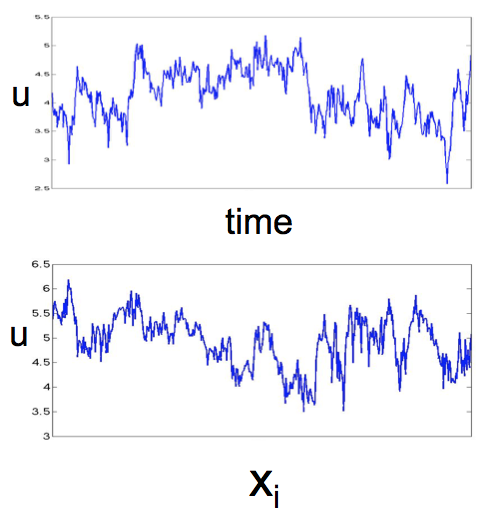
\includegraphics[width=\textwidth]{timetrace2.png}
    \end{column}
    \begin{column}{.35\textwidth}
    \begin{minipage}[c][.7\textheight][c]{\linewidth}
    \begin{itemize}
      \item Unsteady\newline\newline\newline\newline\newline\newline
      \item Three-dimensional	
      \end{itemize}
      \end{minipage}
    \end{column}
  \end{columns}

\end{frame}
%------------------------------------------------

\begin{frame}{Basic Properties of Turbulence}
\begin{itemize}
\item \textbf{Turbulence is random} \newline The properties of the fluid ($\rho$, $P$, $u$) at any given point ($\vec{x}$,$t$) cannot be predicted. But statistical properties – time and space averages, correlation functions, and probability density functions – show regular behavior. The fluid motion is stochastic.
\item \textbf{Turbulence decays without energy input} \newline Turbulence must be driven or else it decays, returning the fluid to a laminar state.
\end{itemize}
\end{frame}

%------------------------------------------------

\begin{frame}{Basic Properties of Turbulence}
\begin{itemize}
\item \textbf{Turbulence displays scale-free behavior} \newline On all length scales larger than the viscous dissipation scale but smaller than the scale on which the turbulence is being driven, the appearance of a fully developed turbulent flow is the same.
\item \textbf{Turbulence displays intermittency} \newline ``Outlier'' fluctuations occur more often than chance would predict.
\item \textbf{Turbulence is non-linear} \newline Growth of small perturbations, non-linear vortex stretching
\end{itemize}
\end{frame}

%------------------------------------------------

\begin{frame}{Basic Properties of Turbulent Flows}
\begin{itemize}
\item Large vorticity\newline\newline
\item Vorticity describes the tendency of something to rotate.
\begin{align*}
\omega &= \nabla \times \vec{u}\\
&= \epsilon_{ijk}\frac{\partial}{\partial x_i}u_j \hat{e}_k\\
&= \left(\frac{\partial u_3}{\partial x_2} - \frac{\partial u_2}{\partial x_3}\right)\hat{e}_1 + \left(\frac{\partial u_1}{\partial x_3} - \frac{\partial u_3}{\partial x_1}\right)\hat{e}_2 + \left(\frac{\partial u_2}{\partial x_1} - \frac{\partial u_1}{\partial x2}\right)\hat{e}_3
\end{align*}
~\\
Vortex stretching can and does create small scale circulations that increases the turbulence intensity $I$, where:
$$I = \frac{\sigma_u}{\langle u \rangle}$$
\end{itemize}
\end{frame}

%------------------------------------------------

\begin{frame}{Basic Properties of Turbulent Flows}
\begin{itemize}
\item Mixing effect\newline\newline
Turbulence mixes quantities (\textit{e.g.}, pollutants, chemicals, velocity components, etc)., which acts reduce gradients. This lowers the concentration of harmful scalars, but increases drag.
\item A continuous spectrum (range) of scales.
\begin{figure}
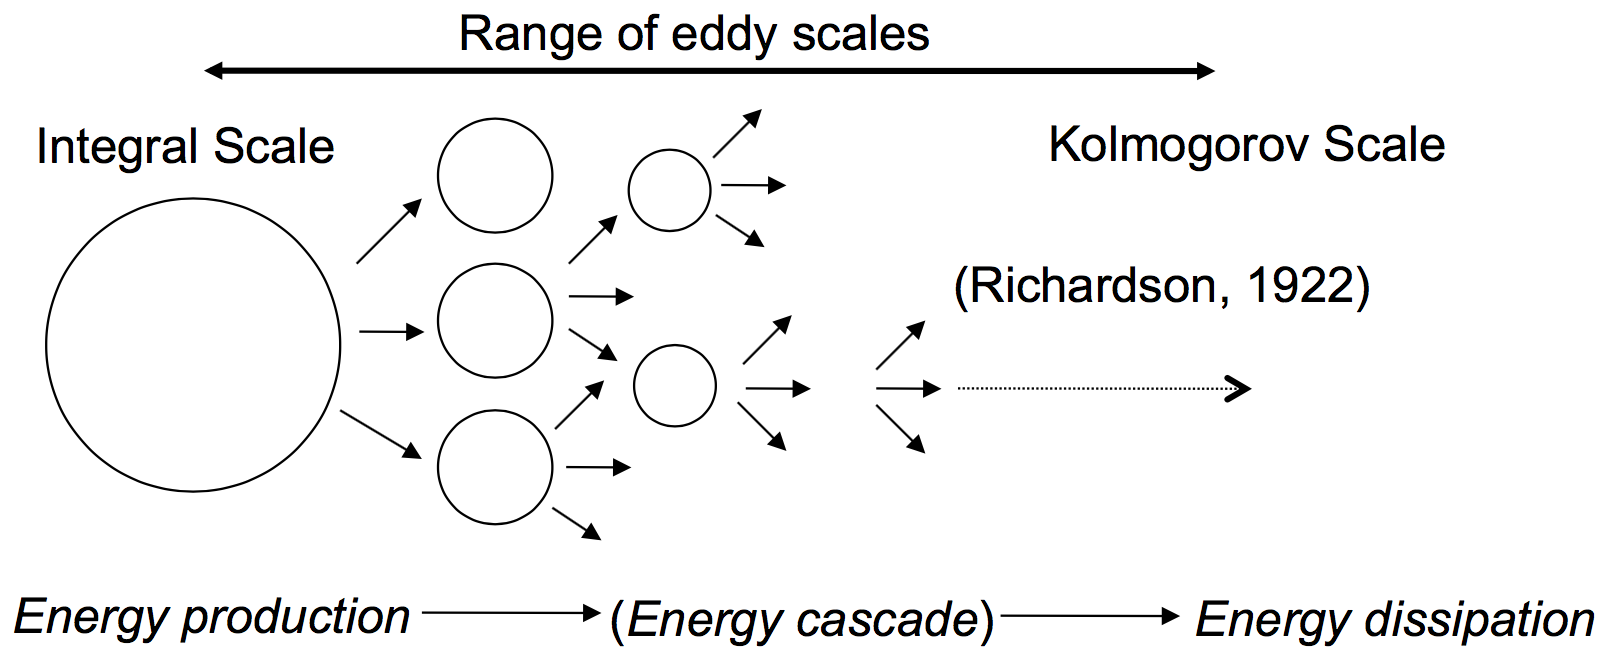
\includegraphics[width=0.9\textwidth]{scales}	
\end{figure}
\end{itemize}
\end{frame}

%------------------------------------------------
\section{Random Nature of Turbulence} %
%------------------------------------------------
\framecard[colorred]{{\color{white}\Huge Random Nature of Turbulence}}
%------------------------------------------------
\begin{frame}{Random Nature of Turbulence}
  \begin{figure}[H]
  \centering
  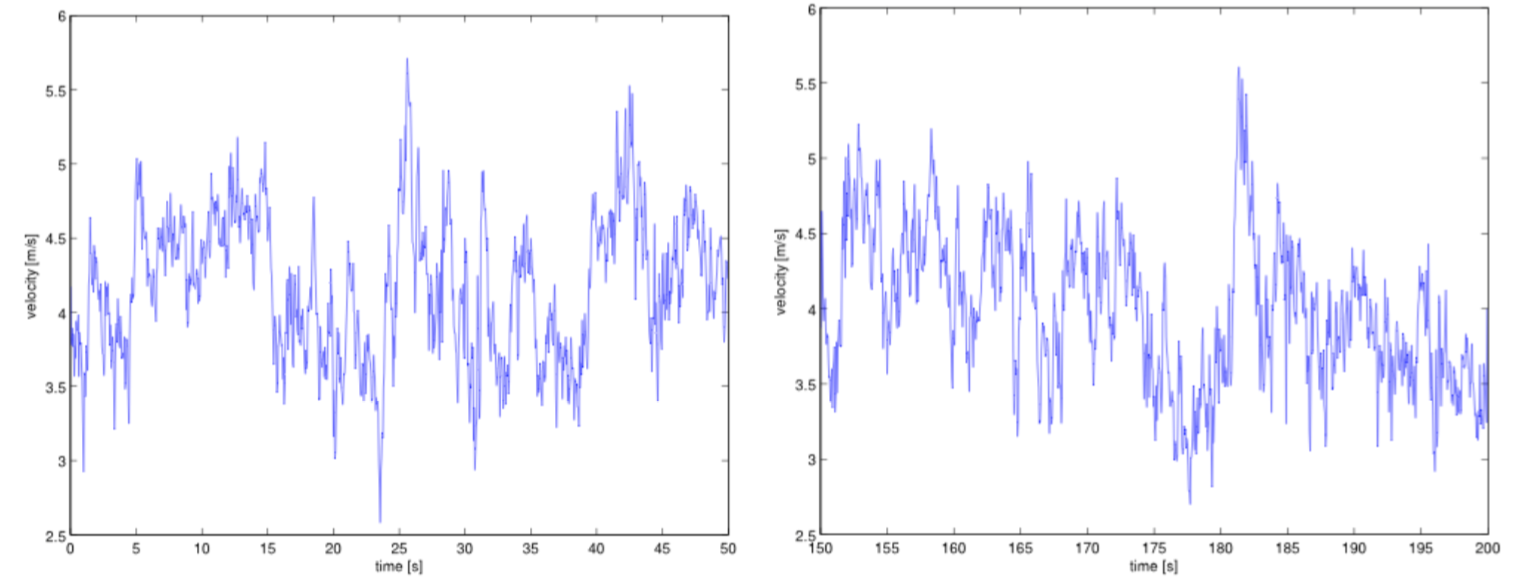
\includegraphics[width=1\textwidth]{timetrace1.png}
  \caption{\scriptsize Sonic anemometer data at 20Hz taken in the ABL.}
  \end{figure}
  
  This velocity field exemplifies the random nature of turbulent flows.
\end{frame}

%------------------------------------------------

\begin{frame}{Random Nature of Turbulence}
  \begin{figure}[H]
  \centering
  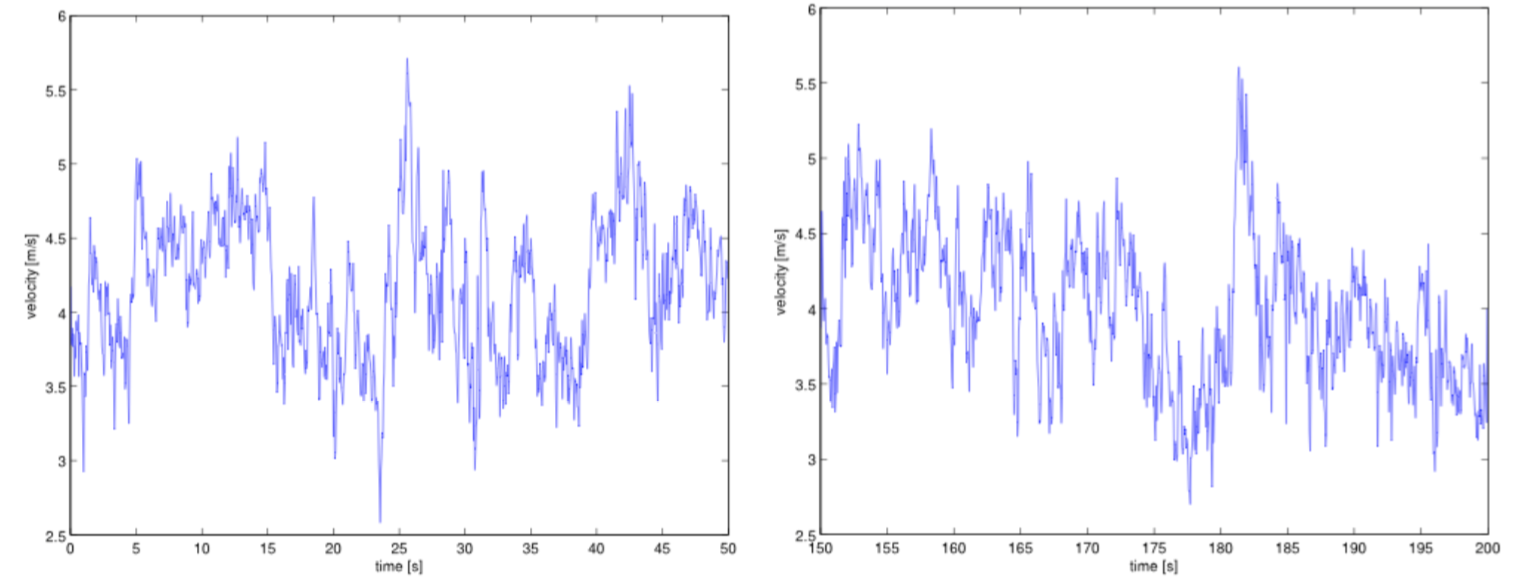
\includegraphics[width=1\textwidth]{timetrace1.png}
  \end{figure}
  \begin{itemize}
  \item The signal is highly disorganized and has structure on a wide range of scales (that is also disorganized).\newline\newline Notice the small (fast) changes verse the longer timescale changes that appear in no certain order.
  \end{itemize}
\end{frame}

%------------------------------------------------

\begin{frame}{Random Nature of Turbulence}
  \begin{figure}[H]
  \centering
  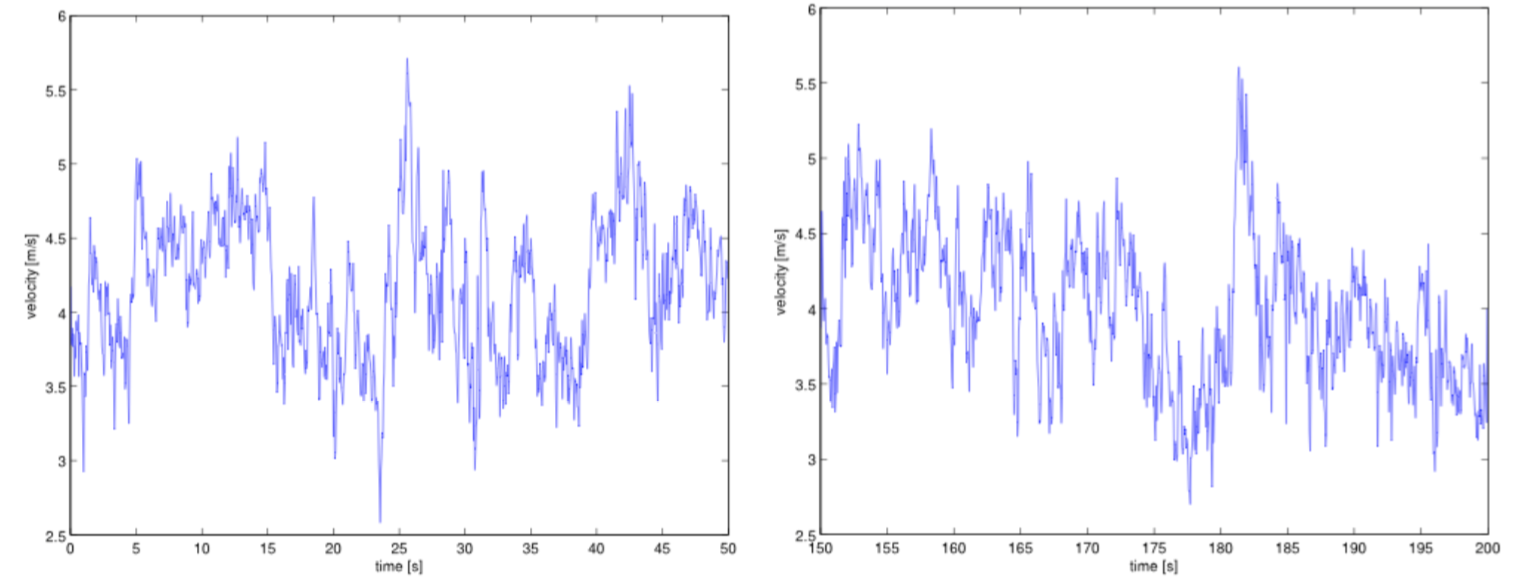
\includegraphics[width=1\textwidth]{timetrace1.png}
  \end{figure}
  \begin{itemize}
  \item The signal appears unpredictable.\newline\newline Compare the left plot with that on the right ($100$ s later). Basic aspects are the same but the details are completely different. From looking at the left signal, it is impossible to predict the right signal.
  \end{itemize}
\end{frame}

%------------------------------------------------

\begin{frame}{Random Nature of Turbulence}
  \begin{figure}[H]
  \centering
  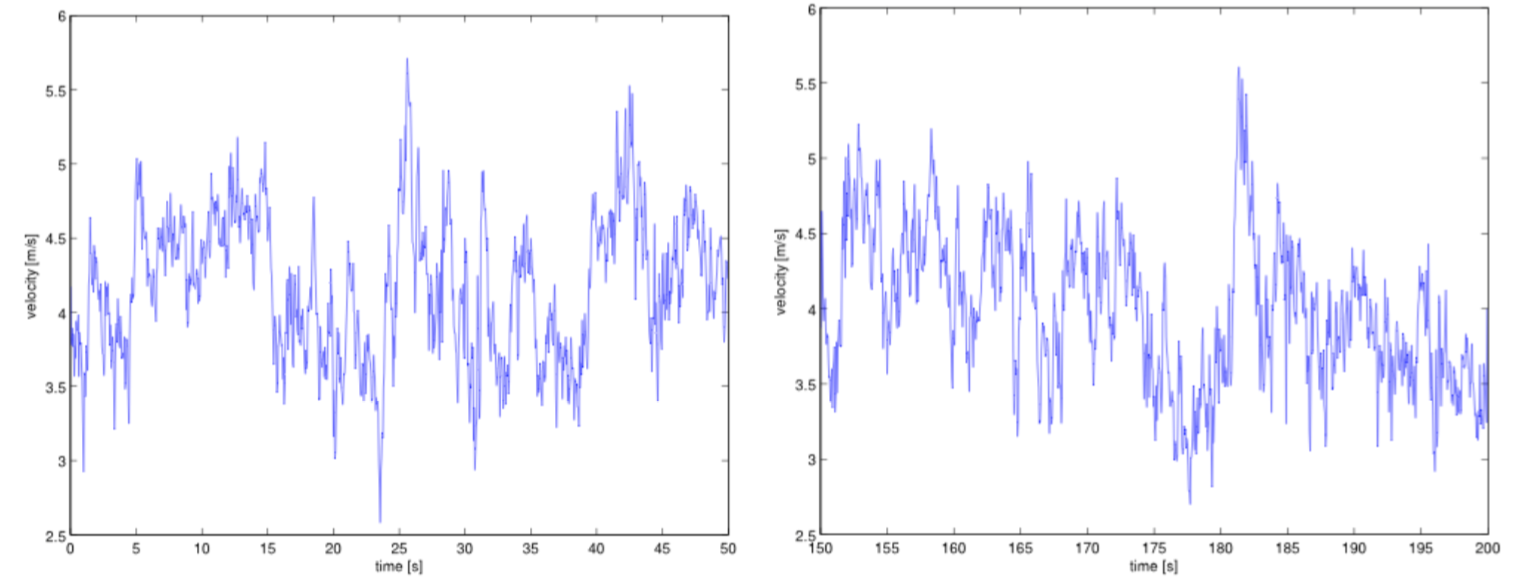
\includegraphics[width=1\textwidth]{timetrace1.png}
  \end{figure}
  \begin{itemize}
  \item Some of the properties of the signal appear to be reproducible.\newline\newline The reproducible property isn't as obvious from the signal. Instead we need to look at the histogram.
  \end{itemize}
\end{frame}


%------------------------------------------------

\begin{frame}{Random Nature of Turbulence}
  \begin{figure}[H]
  \centering
  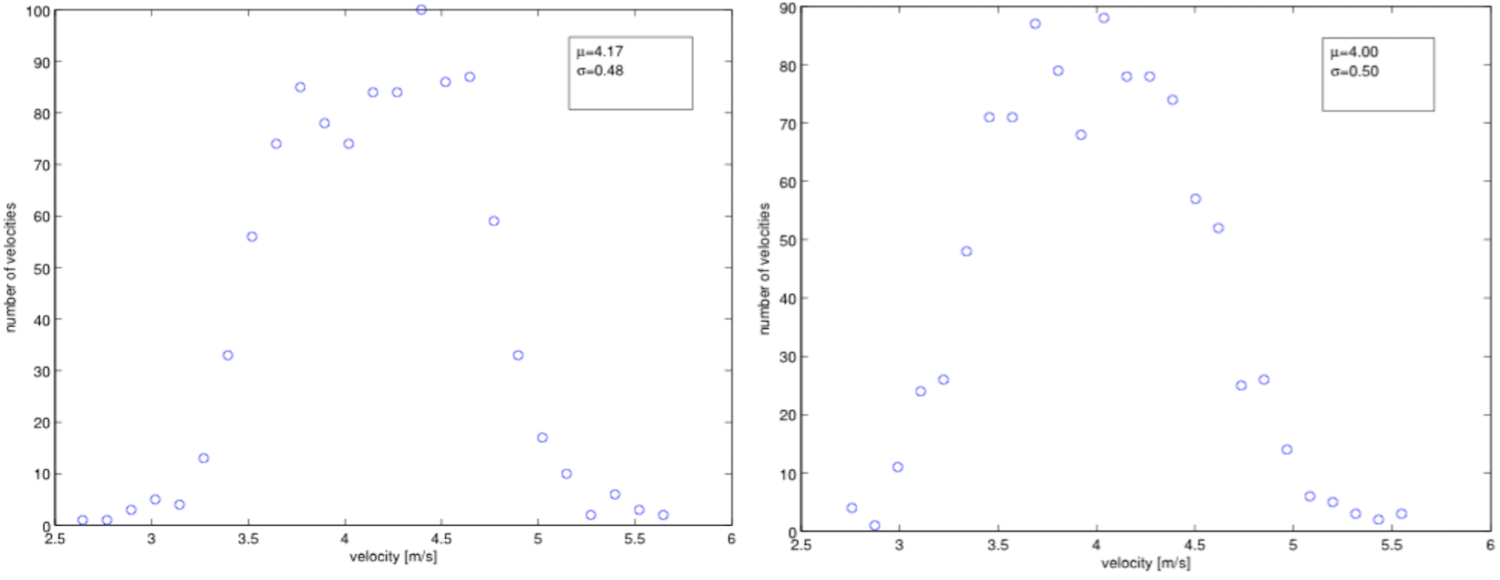
\includegraphics[width=1\textwidth]{histogram.png}
  \end{figure}
  Notice that the histograms are similar with similar means and standard deviations.
\end{frame}

%------------------------------------------------

\begin{frame}{Random Nature of Turbulence}
\setlength{\fboxsep}{0pt}
\setlength{\fboxrule}{1pt}
\begin{columns}[T]
    \begin{column}{.35\textwidth}
      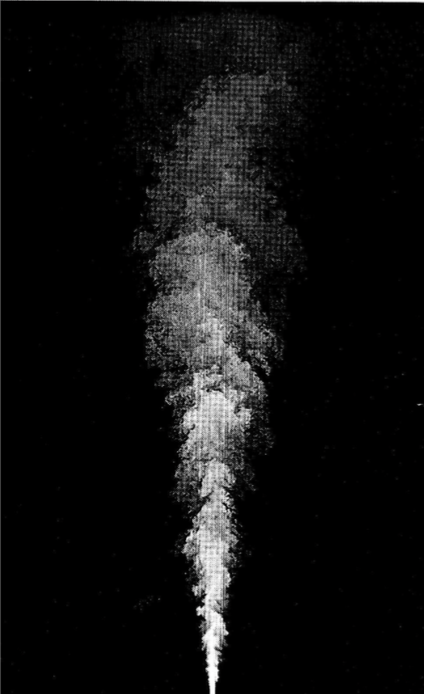
\includegraphics[width=\textwidth]{jet.png}
    \end{column}
    \begin{column}{.65\textwidth}
    \begin{minipage}[c][.7\textheight][c]{\linewidth}
    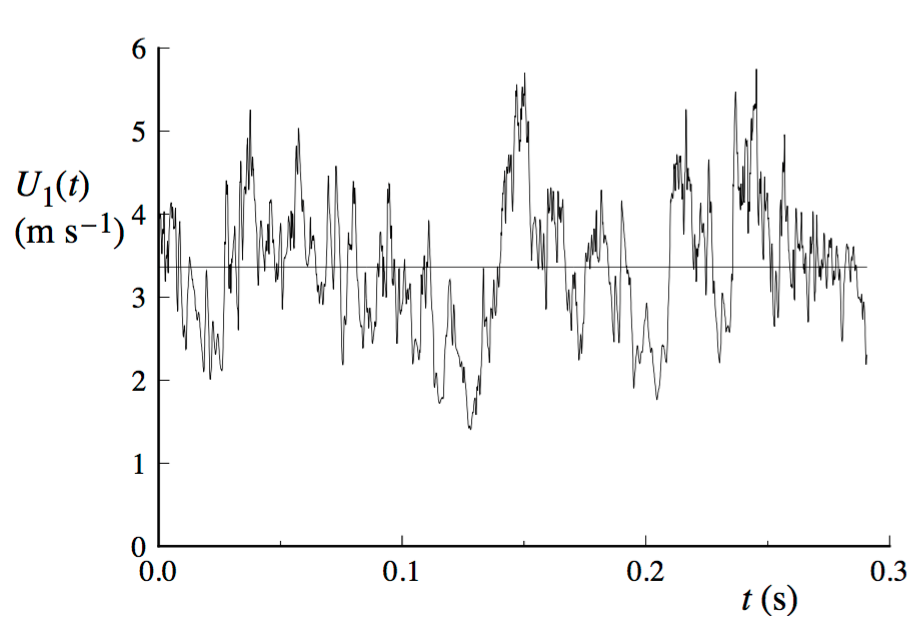
\includegraphics[width=\textwidth]{timetrace3.png}
    \end{minipage}
    \end{column}
  \end{columns}
  The left panel shows concentration in a turbulent jet, while the right shows the time history along the centerline (see Pope).
\end{frame}

%------------------------------------------------

\begin{frame}{Random Nature of Turbulence}
  \begin{figure}[H]
  \centering
  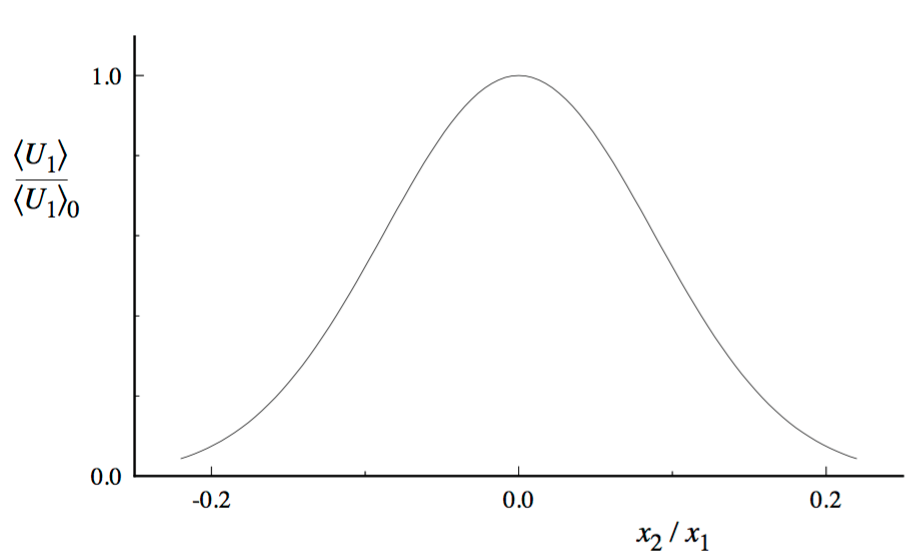
\includegraphics[width=1\textwidth]{crossu.png}
  \end{figure}
  Normalized mean axial velocity in a turbulent jet (see Pope).
\end{frame}

%------------------------------------------------

\begin{frame}{Random Nature of Turbulence}
  \begin{itemize}
  	\item The random behavior observed in the time series can appear to contradict what we know about fluids from classical mechanics.
  	\item The Navier-Stokes equations are deterministic (\textit{i.e.}, they give us an exact mathematical description of the evolution of a Newtonian fluid).
  	\item Yet, as we have seen, turbulent flows are random.
  	\item How do we resolve this inconsistency?
  \end{itemize}
\end{frame}

%------------------------------------------------

\begin{frame}{Random Nature of Turbulence}
  Question: Why the randomness?
  \begin{itemize}
  	\item There are unavoidable perturbations (\textit{e.g.}, initial conditions, boundary conditions, material properties, forcing, etc.) in turbulent flows.
  	\item Turbulent flows and the Navier-Stokes equations are acutely sensitive to these perturbations.
  	\item These perturbations do not fully explain the random nature of turbulence, since such small changes are present in laminar flows.
  	\item However, the sensitivity of the flow field to these perturbations at large Re is much higher.
  \end{itemize}
\end{frame}

%------------------------------------------------

\begin{frame}{Random Nature of Turbulence}
  \begin{itemize}
  	\item This sensitivity to initial conditions has been explored extensively from the viewpoint of dynamical system. This is often referred to as chaos theory.
  	\item The first work in this area was carried out by Lorenz (1963) in the areas of atmospheric turbulence and predictability. Perhaps you have heard the colloquial phrase, \textit{the butterfly effect}.
  	\item Lorenz studied a system with three state variables $x$, $y$, and $z$ (see his paper or Pope for details). He ran one experiment with $x(0) = 1$ and another with $x=1.000001$, while $y$ and $z$ were held constant.
  \end{itemize}
\end{frame}

%------------------------------------------------

\begin{frame}{Random Nature of Turbulence}
  \begin{figure}[H]
  \centering
  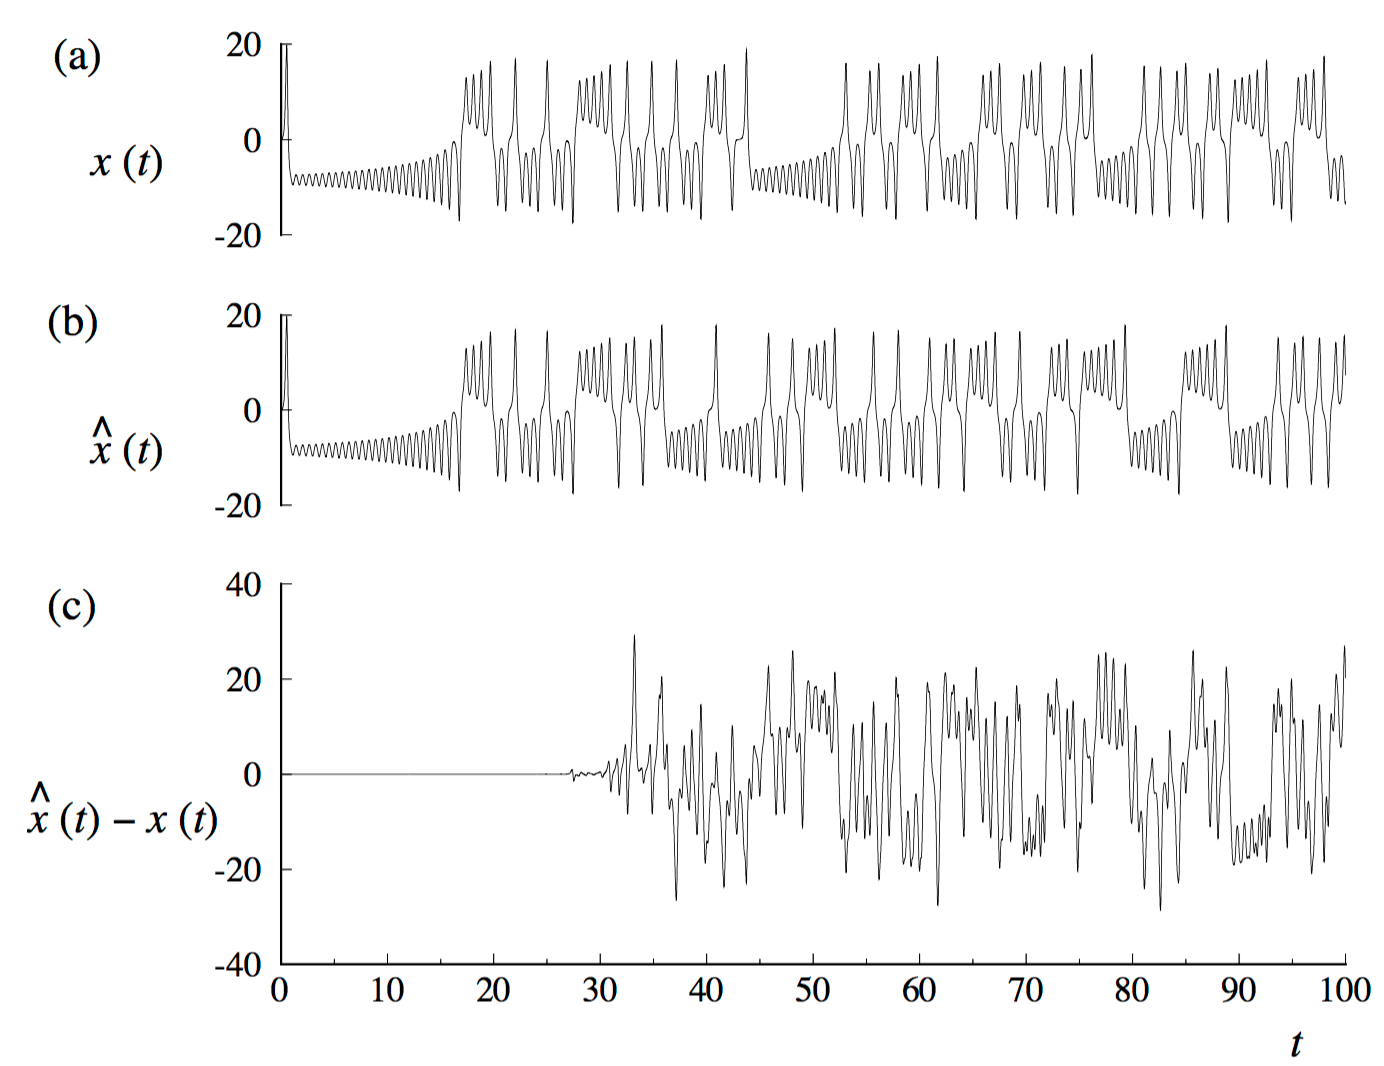
\includegraphics[width=0.85\textwidth]{lorenz.png}
  \caption{Time history of the Lorenz equations.}
  \end{figure}
\end{frame}

%------------------------------------------------

\begin{frame}{Random Nature of Turbulence}
  \begin{itemize}
  	\item The work by Lorenz demonstrates the extreme sensitivity to initial conditions.
  	\item The result of this sensitivity is that beyond some point, the state of the system cannot be predicted (\textit{i.e.}, the limits of predictability).
  	\item In the Lorenz example, even when the initial state is known to within $10^{-6}$, predictability is limited to $t = 35$.
  \end{itemize}
\end{frame}

%------------------------------------------------

\begin{frame}{Random Nature of Turbulence}
  \begin{itemize}
  	\item In the Lorenz example, this behavior depends on the coefficients of the system. If a particular coefficient is less than some critical value, the solutions are stable. If, on the other hand, it exceeds that value, then the system becomes chaotic.
  	\item This is similar to the Navier-Stokes equations, where solutions are steady for a sufficiently small Re, but turbulent if Re becomes large enough.
  \end{itemize}
\end{frame}

%------------------------------------------------

\begin{frame}{Random Nature of Turbulence}
  \begin{itemize}
  	\item We have seen that turbulent flows are random, but their histograms are apparently reproducible.
  	\item As a consequence, turbulence is usually studied from a statistical viewpoint.
  \end{itemize}
\end{frame}

%------------------------------------------------
\end{document}

